% Chapter Template

\chapter{Analysis and Results - Active Monitoring} % Main chapter title

\label{Chapter6} % Change X to a consecutive number; for referencing this chapter elsewhere, use \ref{ChapterX}

\lhead{Chapter 6. \emph{Analysis and Results -  Active Monitoring}} % Change X to a consecutive number; this is for the header on each page - perhaps a shortened title

%----------------------------------------------------------------------------------------
%	SECTION 1
%----------------------------------------------------------------------------------------

%Trying to associate -> rejected some time -> status code = 12 ?
%Connecté et puis disconection abrupte -> code = 3 ?


\section{Analysis}
This chapter focus on the analysis made by our probe. This device simulate a lambda user that tries to get a connection to the UCL's wireless network in order to access the Internet. The procedure followed by the device is quite simple. For each SSID available on the campus, it

\begin{enumerate}
\item associates with the Access Point
\item gets an IP address
\item checks the availability of a set of services
\end{enumerate}

The goal here, it is to get an overview of the infrastructure from the point of view of the user. It is something really interesting because most of the time, the administrators based their diagnostics only on the state of the components that they directly managed. Here, we try to complete those observations by the opposite view i.e. the view of the devices that use the infrastructure.

The purpose of the active monitoring is, as mentioned before, to simulate a user on the network and make a bunch of tests in order to get a live overview of the network status. During the connection loop, a various set of data are gathered and inserted into log files. We have decided to focus on several metrics. As a reminder, here are the information available into a typical log file.

\begin{itemize}
	\item[Scan results] The set of access points around the device and other RF related information.
	\item[AP tried]  The set of access points that the device tries to associate with.
	\item[AP connected] The set of access points that the device has associate with during the tests. As most of the device, our router can choose to change its currently used access point to a better one (i.e roaming).
	\item[Supplication Time] Time elapsed during the connection establishment.
	\item [DHCP Time] Time elapsed till an \texttt{IP} address is assigned to the device.
	\item [Service checks] The results of the service availability tests.
\end{itemize}

Those information will be stored and analysed by the server. By aggregating those data gatherer throughout time, we will build an estimation of the quality experienced by the users.

\section{Scanning}
The first part of the log file aggregates all the scan results performed by the supplicant before connecting to a network. Those information are quite interesting since they allow us to get live details about the current environment of the router. Thanks to those results we have a full overview of the signal strength of all the surrounding access points as well as their frequencies and the \texttt{SSID} they broadcast. 

\paragraph*{Current Wifi Environment} On the interface, we can see the last scan results send by the device. This can help the administrator to diagnostic some \emph{dead zones} on the campus. We have here the view of the device itself and by consequence we can directly tell if the place where the probe is, is correctly covered or not. We could have chosen to plot the signal strength throughout the day but in our situation the RF environment is quite stable and we prefer to provide the most recent scan. Nevertheless, such analysis could be interesting for administrators that desire to monitor a room where the RF conditions significantly vary. All the data required are already available in the database to support that extension.

\paragraph*{Source} The source of those data is \emph{wpa_supplicant} itself. Before any association, the supplicant scan the environnement to detect the reachable access points. Those result are available with the a bunch of related information. A typical scan result look like this:

\begin{figure}[H]
	\begin{itemize}
		\item[BSSID] AB:CD:EF:12:34:56
		\item[Frequency] 2412
		\item[Signal Strength] -40 (dBm)
		\item[SSID] visiteurs.UCLouvain
	\end{itemize}
	\caption{Example of Scan Result}
\end{figure}


\section{Access Points Interactions}
The first step of the user when he wants to connect to the network is to identified himself. All the required commands are automatically handle by the supplicant. Those include the association with the access point and the exchanges required by 802.1x to authenticate with the \emph{Radius}.

\subsection{Access Point Association}
The algorithm used by the supplicant is quite straightforward. It lists the access point that broadcast the requested SSID from the better to the worst and try to associate to them in that order. When it succeed, it starts the authentication with the provided login information.

\paragraph*{Rejection} The first observation we could make was that our device does not always connect with the best access point. In fact, it is rejected by several AP before being able to associate. This is not good as our device is by consequence associated by an access point with a weaker signal. That is a perfect example of why such analyses are useful. With common monitoring tools, we cannot detect such issues because it involves the two parts and the information of all the parts are required to begin an analysis. Here, we can observe the status code \emph{12} which means in the \emph{wpa_supplicant} source code\footnote{ieee802_11_defs.h} \texttt{WLAN_STATUS_ASSOC_DENIED_UNSPEC} (Access Denied Unspecified). Our monitoring tool was able to detect the issue but a deeper debugging on the access point and the device is require to find the precise cause. That is clearly outside the possibilities of our system as it have not directly access to the AP. Nevertheless, we record all the tried access point and are able to provide the quantity of AP that reject the association. With that metric, we are able to tell where that issue occur and where not.

\begin{lstlisting}[frame=single,breaklines=true,caption={Exemple of rejection}]
Trying to associate with XX:XX:XX:XX:XX:XX (SSID='student.UCLouvain' freq=2437 MHz)
CTRL-EVENT-ASSOC-REJECT bssid=XX:XX:XX:XX:XX:XX status_code=12
\end{lstlisting}

\pragraph*{Deconnection} Another problem reported during our analysis was the fact that the device randomly disconnect and reconnect during the test. Even if such behavior is totally normal for a common user, it quite disturbing for our test. Because we make several test, those reconnection interrupt the test and make them running on different access points. Like before, we have recorded the event generated by \emph{wpa_supplicant} and identified the cause. The reported error (\texttt{reason=4}) was a inactivity of the access point. Here again, if such issues want to be diagnosed, deeper access to the infrastructure are required and that is outside the scope of this thesis. For now, we monitor the amount of reconnection during a set of tests and are able to inform the user when they occur.

\begin{lstlisting}[frame=single,breaklines=true,caption={Example of Deconnection trace}]
CTRL-EVENT-DISCONNECTED bssid=XX:XX:XX:XX:XX:XX reason=4
Trying to associate with XX:XX:XX:XX:XX:XX (SSID='student.UCLouvain' freq=2437 MHz)
\end{lstlisting}

\paragraph*{Source} All that logs are generated by \emph{wpa_supplicant} and provided through an events generator mechanism. Our program is interface with it and is able to record all those events. Those offer a rich source of information to trace all the steps of the association.

\section{Time Durations}
Time is an important factor when dealing with wireless networks performances. Indeed, the users can be really annoyed when the connection establishment duration begins to take too much time. We have decided to keep track of the time duration it takes for \texttt{wpa\_supplicant} to establish a connection with the network. Concretely, we start a timer when the command \texttt{SELECT\_NETWORK} is sent to the control interface to start the connection phase and we stop it as soon as a \texttt{WPA-EVENT-CONNECTED} is received. We keep track of the time it takes for the \texttt{DHCP} server to provide an \texttt{IP} address to the supplicant as well. The methodology is the same as the one used for the connection establishment's duration computation. A timer is started as soon as the interface is connected to the network and before sending a \texttt{DISCOVER} message to the \texttt{DHCP} client, and is stopped as soon as a lease for an \texttt{IP} address is obtained. 

\pragraph*{Decomposition} An interesting feature of this analysis is that we can decompose the waiting time of the user in different steps. By observing the proportion of each steps, we could point what steps constitute the bottleneck of the connection. As we observe those indicators during several hour, we can monitor their evolution make the distinction between persistent problems and the isolated cases. After gathering data and plotting them on a graph, we have come to conclusion that, despite the fact that we sometimes have peaks in the duration, the connection and \texttt{DHCP} times remain rather constant. Here is an example for the networks \texttt{UCLouvain-prive} and \texttt{UCLouvain} record from the \emph{Reaumur} building.

\begin{figure}[H]
	\centering
   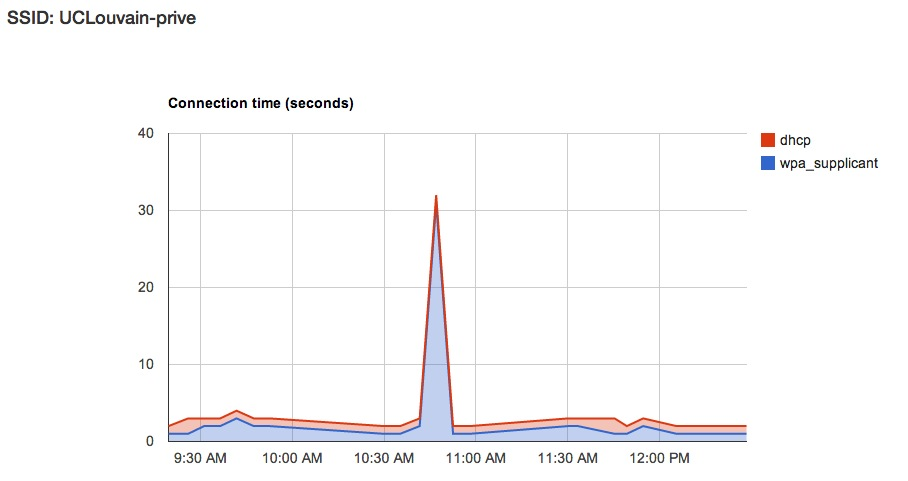
\includegraphics[width=1\textwidth]{Pictures/chapter6/time-uclouvain-prive.jpg}
   \caption{Connection time for \texttt{UCLouvain-prive}}
\end{figure} 

\begin{figure}[H]
	\centering
   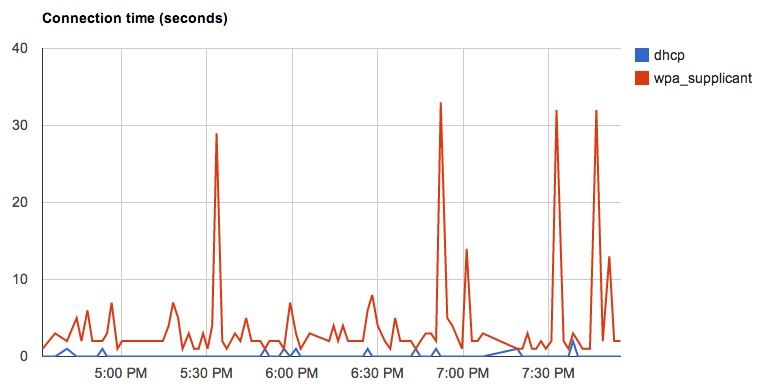
\includegraphics[width=1\textwidth]{Pictures/chapter6/time-uclouvain.jpg}
   \caption{Connection time for \texttt{UCLouvain}}
\end{figure} 

\pragraph*{Peak of time} We have investigated on the possible reasons of those peaks and we have noticed that the \texttt{wpa\_supplicant} daemon seems to spend a lot of time in the association phase. As said before, AP is sometimes rejecting the device and force the supplicant to try with other ones. This may induce some latency in the connection phase and impact the experience of the user. In order to understand why those rejected association happen, we checked the log file of the \texttt{WiSM} and we found a lot of times the same \texttt{LWAPP} error message.\\
\begin{lstlisting}[frame=single,breaklines=true,caption={\texttt{WiSM} association error message}]
%LWAPP-3-INVALID_AID2: Association identifier [int] for client [hex]:[hex]:[hex]:[hex]:[hex]:[hex] is already in use by[hex]:[hex]:[hex]:[hex]:[hex]:[hex]
\end{lstlisting}

The explanation\footnote{http://www.cisco.com/c/en/us/td/docs/wireless/controller/message/guide/controller\_smg/msgs6.html} \texttt{Cisco} gives for that message is that an internal error caused an invalid association ID to be received from an AP for the indicated client and that the client may experience communications problems. This issue can be observed with other device on the network and could be linked to the fact that we generate a lot of association in a short time.

\paragraph*{Source} This analysis heavily use the event mechanism of \emph{wpa_supplicant} to generate its estimations of duration. We complete the analysis with the controller logs which are available on the \emph{Gathering} part. This is also a good example that a system embedding all the monitoring tools could help to generate better analysis about issues on a complex infrastructure.


\section{Services Availability}
We wanted our application to be able to give a performance and quality overview of the network every time a new connection is established. As mentioned before, we have divided our test into two parts. First we perform a \texttt{DNS} query on the two \texttt{DNS} servers of the UCL to see if both servers are reachable. Then we test the \texttt{TCP} connection to the main UCL's services added to the collection of the ten most visited website in the world with simple \texttt{socket} connections. After having received several log files from the router we were able to check the results and make some analysis on them. 

\pragraph*{DNS} First of all, both \texttt{DNS} servers are always reachable and accessible for the five \texttt{VLANs}. The interest here come from the fact that for the users, when the DNS does not work, it the same that the \emph{internet} does not work. By decoupling those analysis, we can localize more precisely the connectivity issues.

\pragraph*{Service checks} Then, the results of the service reachability test depends on which network the test is executed. Indeed, the UCL's online wireless documentation states that some \texttt{VLANs} restrict the range of websites accessible. We were able to confirm that information thanks to our system. Upon our analysis we can see that, only two networks have some restrictions.
\begin{itemize}
	\item [-] \texttt{visiteurs.UCLouvain}
	\item [-] \texttt{UCLouvain-prive}
\end{itemize}
The choice of the checked service is quite simple. We start by enumerating all the UCL related service that a typical student need to access for his courses. The exhaustive list is available in the Chapter 4. By checking periodically those services, we can generate their rate of availability which can be a good indicator to determine the quality perceived by the user.

\paragraph*{Source} The data used in these analysis are completely generated by our system. The test are performed by sub routines implemented in our \emph{OpenWRT} script. All the information are centralized in the server and the analysis are performed on it.


\section{Limitations}
The main limitation of those analysis is the interface of \emph{wpa_supplicant}. We interface our program with and use its message and functions to generate our data. A more powerful approach would be to work directly in the \emph{wpa_supplicant} code and extent it with our program. That is far more complex and would require a lot more of time. Nevertheless, it is really an interesting idea for future extensions for our system.

\section{Summary}
In this chapter, we have presented some analysis performed by our simulator of user. Even if this prototype implements some limited features, we think that they demonstrate that they can really help to diagnostic more subtle issue in the network. Having that double view of the network (i.e. Controller and User) can lead to a new way of diagnostic a complex infrastructure.

